%\section{Visual Analysis Requirements and Overview of Our Approach}

\section{Design Goals}
\label{sec:goals}
% \TF{(1) We should think a good way to link the issues (mentioned in Intro and Background) and design requirements. (2) We should clarify which part of the workflow or the view is developed to address each issue. (3) We should link the workflow and the system view as well (i.e., put some labels (e.g., a, b, c) on the workflow and the system). (4) the workflow section should show the simple scenario to make the entire process easy to understand. For example, we can show how we reach the state shown in Fig. 2.}

% The aforementioned problems with the analysis of neurodegenerative diseases have led us to design a new method with a list of visual analysis requirements. Next, we will describe those requirements and then present an overview of our approach. 

% To develop a system which solves the problems described in \autoref{sec:problems}, we identify several key design requirements. DG1 and DG2 correspond to Problems 1 and 2 in \autoref{sec:problems}, respectively. 
% DG3 and DG4 are to solve Problem 3.\\
% Also, we introduce a visual analytic workflow to that suppports an analysis which follows all the requirements.

% \begin{figure*}[tb]
%     \centering
%     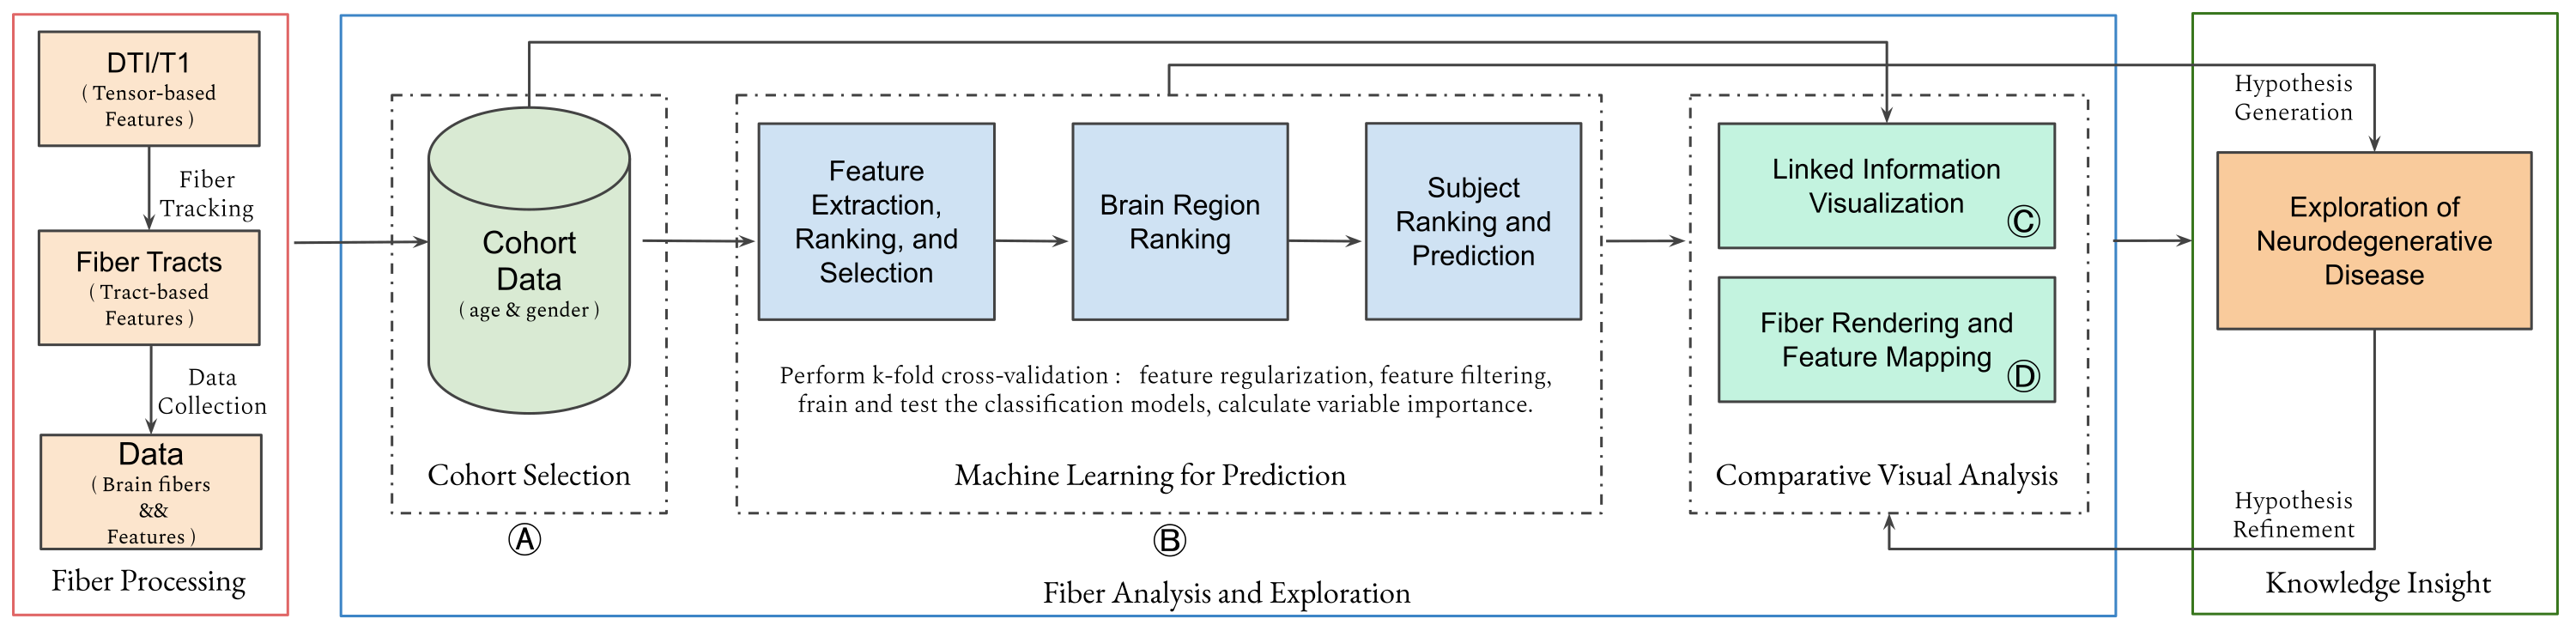
\includegraphics[width=1.0\textwidth]{images/Vis2020_Workflow.png}
%     \caption{A Schematic Diagram of the visual analytics process.}
%     \label{fig:workflow}
% \end{figure*}


%SystemVersion2.png
\begin{figure*}[ht]
    \centering
    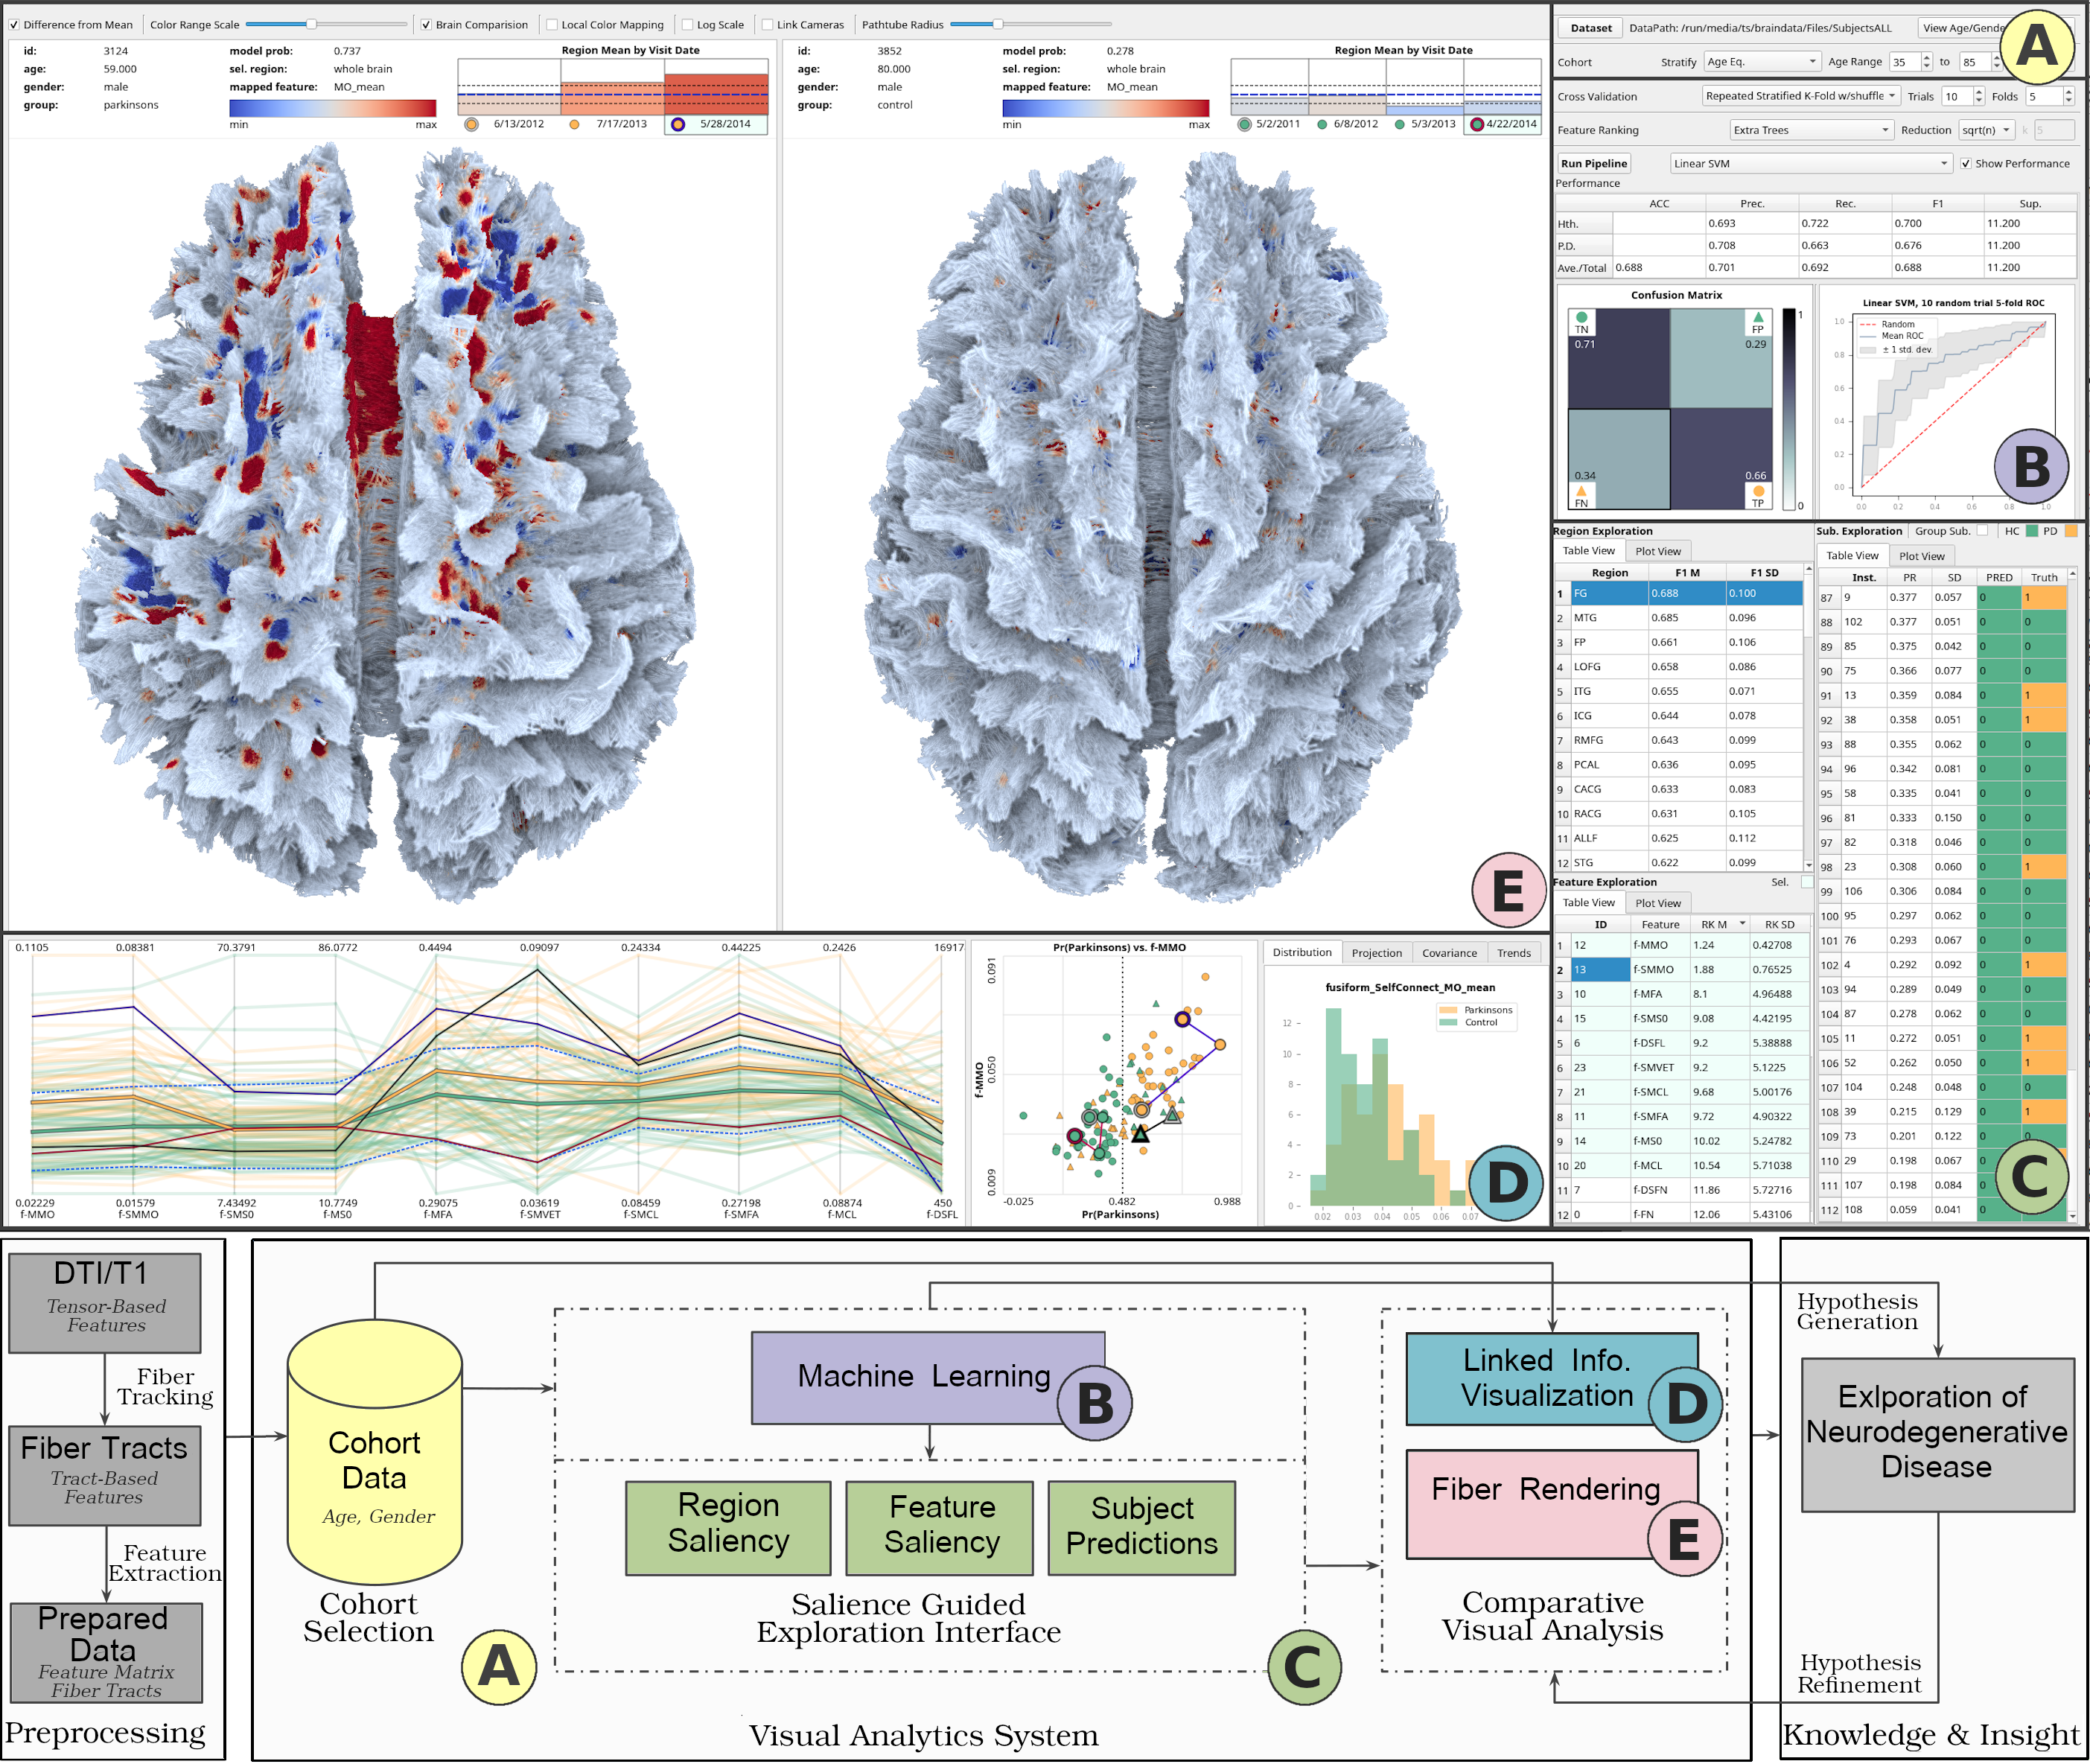
\includegraphics[width=0.99\textwidth]{images/SystemVersion2.png}
    \caption{The UI of our visual analytics system. \clc{A} The cohort selection module supports balanced and stratified subject group selection and demographic analysis. \clc{B} The ML module can be customized before executed. The results (below) summarize the model performance and overall uncertainty. This includes an ROC curve, confusion matrix, the group sizes, and 4 difference performance measures: accuracy, precision, recall, and $F_1$. \clc{C} The interface for exploration includes 3 sub-modules: the region module, feature module, and subject module. They can each be toggled between plot views and table views as described in further sections. The values displayed include averages and standard deviations of the estimated silences and predictions. The subject view also encodes the class labels and binary predictions. \clc{D} The information visualization module includes a range of views for comparative analysis. \clc{E} The 3D fiber rendering views show selected subjects for physiological analysis.  The selected feature is mapped to the fibers through color; in this case a divergent color map is used and the mapped values represent the difference from the mean of the control group. Above each fiber view shows subjects' information and a timeline showing their mean values of the selected feature over time. The intervals on the timeline can be clicked to change the fiber view to display those different scans. Above the fiber views are adjustable rendering and viewing parameters, such as path tube thickness, camera linking, logarithmic scaling, and constrastive or direct value mapping.
    }
    \label{fig:system}
\end{figure*}

The aforementioned problems in neurodegenerative disease research have inspired the design goals for our system. 
Using our teams expertise (which includes machine learning, visual analytics, and fiber tract visualization), we made a prototype system.
% With the expertise of a researcher that has some prior experience studying fiber tracts in an interdisciplinary lab, we made a system prototype. 
Then, we consulted five experts in different research fields, including statistical analysis of neurodegenerative disease, brain tractography of MRI images, and diagnosis and treatment of PD. While consulting the neuroscientists, they gave us feedback based on their unique perspectives and backgrounds. We then improved the system according to their feedback. The design goals are as follows: 

%The aim of this phase is to identify design goals of our system. We worked closely with five experts (two academic scholars at universities and three clinicians at hospital) with unique perspectives and backgrounds in neuroscience, including statistical analysis of neurodegenerative disease,  brain tractography from MRI images, diagnosis and treatment of PD. We have several round discussions from creating a common understanding between visualization scientists and the neuroscientists to iteratively designing the system based on the experts' suggestions. The distilled design goals for the brain fiber data analysis system are as follows: 

%The aforementioned problems in neurodegenerative disease research have inspired us to design goals for our system. With the experience of the researcher that has been working on brain fiber analysis in neurodegenerative disease for multiple years, we identified the design goals. While consulting neuroscientists in different research fields (e.g.,  PD and AD), they feel the design goals were reasonable and well worth the effort.
    
\begin{asparadesc}

    \item[DG1] \textbf{Guided analysis based on 3 modalities.}
   To facilitate an effective workflow, our system should help the user prioritize more salient (\textbf{a}) regions, (\textbf{b}) features, and (\textbf{c}) to pragmatically choose subjects for detailed analysis. \textbf{d}. The regions and features should be standard and interpretable so that experts can more easily grasp the physiological basis, assimilate existing literature, and make hypothesis. \textbf{e}. Due to a large feature space relative to the number of scans, we must strive to avoid overfitting, reduce ranking instability, and highlight the uncertainties.
    
    % A large amount of features (e.g., hundreds of features) can be extracted from the whole brain for analyzing neurodegenerative disease. 
    % Therefore, a system should be able to suggest which features and brain regions have significant differences in the diseased brain when compared with the healthy brain. 

	\item[DG2] \textbf{Quality visualization of brain fibers.}
	For anatomical understanding, visual analysis of the fiber tracts and salient variables in the physical space is required. The rendering should be effective at showing structure, while also efficient enough to interactively render multiple large fiber sets simultaneously.
	
	\item[DG3] \textbf{Modalities for comparison.} Besides the explorative modalities that zero in on objects of interest, there are also multiple modalities for comparison of those interesting objects. These comparisons can help experts to relate the diverse and uncertain data in support of hypothesis development. 
%through the cohort study between diseased and healthy brains, 
	Targets for comparison include: group trends, group trends vs. individuals, multiple individual subjects, individual subjects over time, and correlations between variables. Furthermore, since we explore these facets based on estimated salience, we should also highlight their relationships to the driving predictive models. 

    % \item[DG4] \textbf{ Easy-to-use interactions with complex multi-faceted data.}
    \item[DG4] \textbf{Easy non-linear exploration.}
    Due to the large number of features, fiber tracts, and subjects, 
    diverse aspects could be explored. 
    The analytical process may proceed and change according to different patterns that emerge or knowledge that is discovered during the analysis. 
    Therefore, our system should provide an intuitive and fully interactive UI to serve the neuroscientists' changing analytics needs.

% The following DGs (DG1--DG4) are identified to solve the problems described in Sec.~\ref{sec:problems}.
% DG1 and 2 correspond to Problems 1 and 2 in \autoref{sec:problems}, respectively. 
% DG3 and 4 are to solve Problem 3.\\

% \begin{compactdesc}
%     \item[DG1] \textbf{Identification of the most impactful features and brain regions to the disease.}
%     A large amount of features (e.g., hundreds of features) can be extracted from the whole brain for analyzing neurodegenerative disease. 
%     %They may affect the disease to varying degrees. 
%     Therefore, a system should be able to suggest which features and brain regions have significant differences in the diseased brain when compared with the healthy brain. 
	
% 	\item[DG2] \textbf{Quality visualization of the brain fiber tracts.} 
% 	To help anatomical understanding of the disease, visual comparison of the fiber tracts between the diseased and healthy brains is required as well as comparison with statistic features. 
% 	Thus, a system should provide a high quality 3D visualization of the fiber tracts in a user-selected brain region.
% 	%A spatial region based analysis which combines 3D rendering of brain regions with statistic measurements of interest that selected by users mapped to the physical structures would help in an anatomical understanding of the disease. 
	
% 	\item[DG3] \textbf{Overview of relationships between subjects and features.} 
% 	To build a hypothesis through the cohort study between the diseased and healthy brains, a system should provide a visualization of the relationships between subjects and the extracted features. 
% 	Because there will be potentially many different subjects and features, the visualization should provide an overview of the relationships based on the user's need.
% 	%The measurements, to a large extent, can be used to analyze the disease, however, it lacks of gaining the relationship between variables as well as it lacks the overall trends in all the subjects. 
% 	%An overview of all the subjects and distribution of the variables that have a profound impact on the disease can help in the understanding of both the disease and the healthy groups. 
	
% 	%\item[DG4] \textbf{Comparison across subjects and different time steps of a subject.} Although the physical structures and variables can be well observed and understood, researchers cannot make any judgments about the disease without comparison. The comparison between different subjects and different time steps of a specific subject allow researchers discovering the laws of the disease and judging the disease more reasonably. 

%     \item[DG4] \textbf{ Easy-to-use interactions with the complicated data.}
%     Due to the large number of features, fiber tracts, and subjects, there is a wide variety of aspects that could be explored. 
%     The analytical process may proceed and change according to different patterns that emerge or knowledge that is discovered during the analysis. 
%     Therefore, a system should provide an intuitive and fully interactive UI to serve the neuroscientists’ ever-changing analytics needs.
    
% 	Because neurodegenerative disease usually changes over time and it also manifests in individual differences. An observation of per subject trends of disease progression is needed. Furthermore, simply by observing the progressive changes of specific subject in disease will lead to inaccurate judgment. Comparison of measurements across subjects or groups is required. 
%	\item avoid over-fitting and generalization error 
% it seems like the simplest way to increase stability of feature selection is to use something like Random Forrest or other ensemble based methods. This is already implemented in Sci-Kit learn as well. The other recommendation is to group correlated features, or remove redundant ones. It would be nice to handle that, but dealing with feature groups requires more work and features in our system for visualizing and analyzing these groups. For now I will just switch to some ensamble methods. In the writing, I will list 3 requirements (1) account for the selection bias problem inherent in high dimensional data such as ours. (2) Account for selection/ranking stability (for features, subject predictions, brain regions). (3) Avoid pitfalls of circular analysis. We could possibly add these requirements to the existing requirements section, as well.
\end{asparadesc}

